\section{独立测试与结果分析}
\subsection{测试设置与评价方法}

独立测试需要把预测结果和人工标签放在同一位置比较。这里首先核对样本编号、原图和标签的配对关系，再沿用第~\ref{sec:labeldefinition} 节的标签定义生成二值真值与有效区域，眼镜区域不参加评价。

测试使用固定划分中的 32 张图，每张图为 $512\times512$，共有 8,388,608 个有效像素。两套方案使用相同原图、真值和有效区域。检测程序根据原图、训练统计和固定配置生成预测，评价程序再读取保存的预测进行评价。这样可以直接检查最终交付的掩膜是否与对应的真值对齐。

TP 表示脸部像素被正确检出，FP 表示非脸部被错检为脸部，FN 表示脸部被漏掉，TN 表示非脸部被正确排除。各图计数累加后计算式~\eqref{eq:metrics} 中的五项指标。
\begin{equation}
\begin{aligned}
\mathrm{Accuracy}&=\frac{TP+TN}{TP+FP+TN+FN},\\
\mathrm{Precision}&=\frac{TP}{TP+FP},\qquad
\mathrm{Recall}=\frac{TP}{TP+FN},\\
\mathrm{F1}&=\frac{2TP}{2TP+FP+FN},\qquad
\mathrm{IoU}=\frac{TP}{TP+FP+FN}.
\end{aligned}
\label{eq:metrics}
\end{equation}

Precision 说明选出的区域有多少真正属于脸部，Recall 说明真实脸部找回了多少。F1 综合这两类错误，IoU 则直接描述预测区域与真值的重合程度。当前图像中非脸部像素较多，所以以 F1 和 IoU 为主要结果，再结合 Precision、Recall 解释改善来自哪里，Accuracy 作为补充。

\subsection{基线与最终方案的测试比较}

\begin{table}[H]
\centering
\small
\caption{32 张测试图的总体评价结果，单位为百分比}\label{tab:testmetrics}
\begin{tabular}{lrrr}
\toprule
指标 & 纯阈值基线 & 最终方案 & 变化，百分点 \\
\midrule
Accuracy & 76.53 & 83.94 & +7.41 \\
Precision & 52.91 & 66.43 & +13.52 \\
Recall & 76.82 & 75.55 & -1.27 \\
F1 & 62.66 & 70.69 & +8.03 \\
IoU & 45.63 & 54.67 & +9.04 \\
\bottomrule
\end{tabular}
\end{table}
\begin{table}[H]
\centering
\small
\caption{测试集混淆计数}\label{tab:testcounts}
\begin{tabular}{lrrrr}
\toprule
方案 & TP & FP & TN & FN \\
\midrule
纯阈值基线 & 1,652,227 & 1,470,496 & 4,767,390 & 498,495 \\
最终方案 & 1,624,818 & 821,271 & 5,416,615 & 525,904 \\
\bottomrule
\end{tabular}
\end{table}

表~\ref{tab:testmetrics} 中，最终 F1 从 62.66\% 提高到 70.69\%，IoU 从 45.63\% 提高到 54.67\%。变化最明显的是 Precision，它提高了 13.52 个百分点，而 Recall 下降了 1.27 个百分点。

接着看具体计数，FP 减少了 649,225 个像素，FN 增加了 27,409 个像素，所以整体收益主要来自减少误检。最终方案选出的区域更集中，但也舍弃了部分真实脸部。此时只看掩膜是否干净还不够，需要结合真值检查被删除的部分。

\subsection{各处理步骤如何形成最终结果}

基线和最终方案同时改变了颜色阈值和后处理，进一步按执行顺序拆开，可以看到各步骤分别留下了什么。表~\ref{tab:stages} 使用同一批测试图，其中中间两行用于解释流程。

\begin{table}[H]
\centering
\small
\caption{固定流程各阶段的测试结果，指标单位为百分比}\label{tab:stages}
\begin{tabular}{lrrrrr}
\toprule
阶段 & Precision & Recall & F1 & FP & FN \\
\midrule
基线阈值，$k=1.50$ & 52.91 & 76.82 & 62.66 & 1,470,496 & 498,495 \\
颜色阈值，$k=1.25$ & 56.59 & 65.24 & 60.61 & 1,076,315 & 747,523 \\
保留最大连通域 & 64.73 & 63.36 & 64.04 & 742,515 & 787,938 \\
填孔后的最终结果 & 66.43 & 75.55 & 70.69 & 821,271 & 525,904 \\
\bottomrule
\end{tabular}
\end{table}

先把 $k$ 从 1.50 缩小到 1.25，去掉了 394,181 个误检像素，也丢掉了 249,028 个原来检对的脸部像素。颜色范围变严格后，Precision 稍有上升，Recall 明显下降，F1 也随之降低。因此，最终方案的提升需要连同后处理一起解释。

保留最大连通域又去掉了 333,800 个误检像素，同时损失 40,415 个正确像素。这一步更有效地排除了与主体分离的干扰，F1 回升到 64.04\%。接着填孔补回 262,034 个正确像素，并增加 78,756 个误检像素，F1 达到最终的 70.69\%。

这里可以看出这条流程的衔接关系。较严格的阈值先减少候选，最大连通域保留其中较集中的区域，填孔再恢复内部缺失。前面的选择会影响后面的恢复效果，所以还需要结合具体图像检查。

\subsection{成功与失败样例}

以下选取最终 F1 最高、提升最多、下降最多和 Precision 最低的测试样例。误差图中绿色表示正确检出的脸部，红色表示误检，蓝色表示漏检。

00610 的原始候选已经形成了较完整的面部区域，如图~\ref{fig:test610} 所示。$k=1.25$ 时共有 80,328 个候选像素，最大连通域保留了其中的 79,899 个，区域选择只损失 110 个正确像素。随后填孔补回 9,490 个正确像素，最终 F1 为 0.930，Recall 为 97.73\%。该图的脸部主体连贯，缺失又大多被轮廓包围，正好符合这套处理的条件。

\begin{figure}[H]
\centering
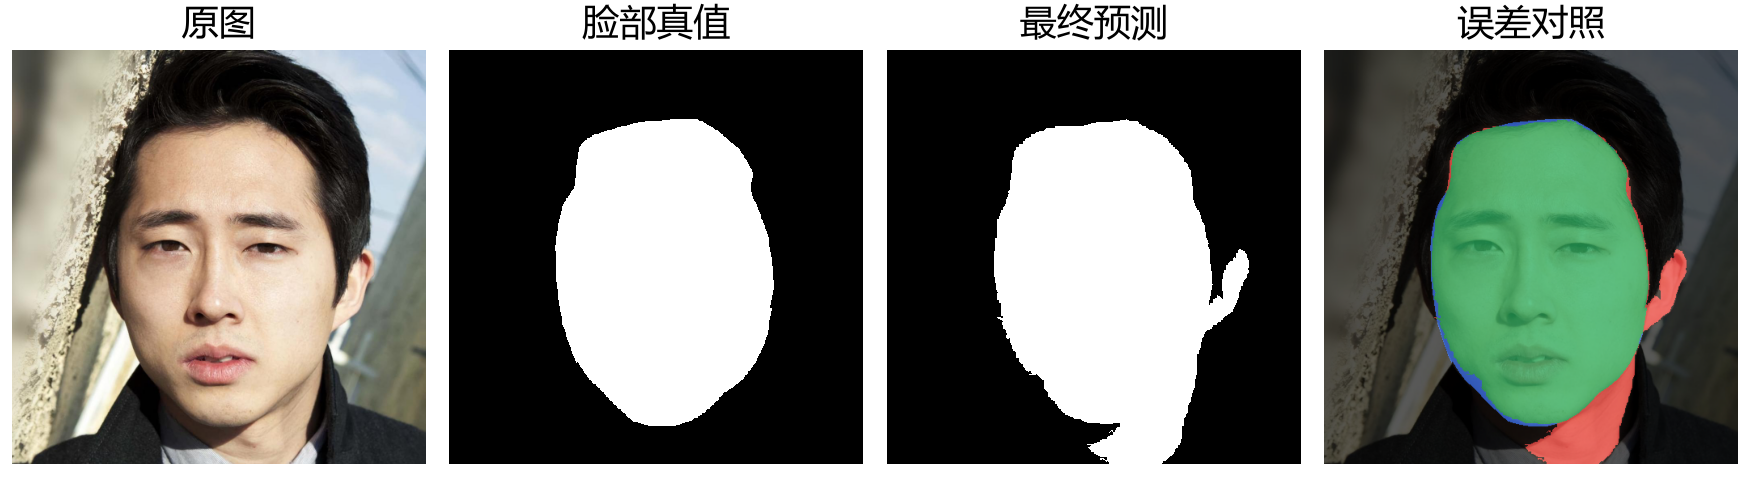
\includegraphics[width=\textwidth]{test_00610.png}
\caption{00610 的原图、真值、最终预测与误差对照}
\label{fig:test610}
\end{figure}

00570 则更能体现最大区域筛选的作用，如图~\ref{fig:test570} 所示。该步骤去掉了 39,579 个误检像素，只损失 939 个正确像素，再通过填孔补回 9,954 个正确像素，F1 从基线的 0.476 提高到 0.759。这说明区域筛选在候选主体合适时，可以有效去掉大片干扰。
\begin{figure}[H]
\centering
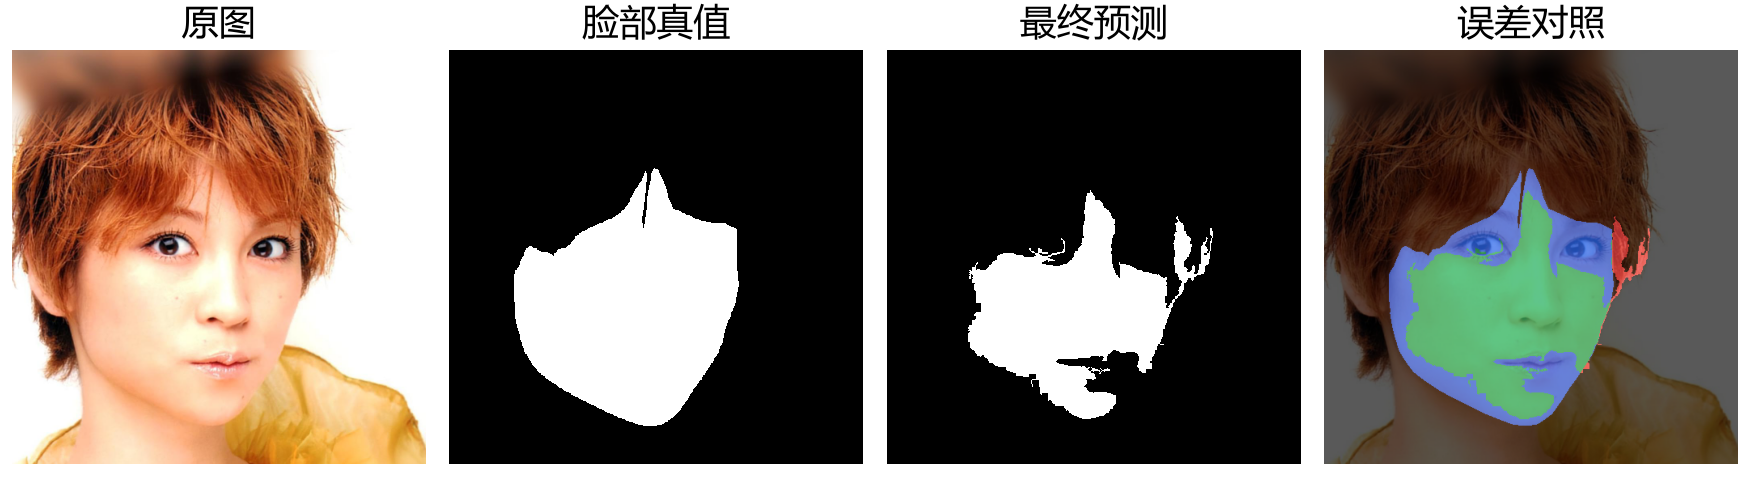
\includegraphics[width=\textwidth]{test_00570.png}
\caption{00570 的原图、真值、最终预测与误差对照}
\label{fig:test570}
\end{figure}

00609 的问题在颜色筛选时已经出现，如图~\ref{fig:test609} 所示。$k=1.25$ 后只剩 5,685 个候选像素，覆盖真实脸部的 8.33\%，并分成 56 个连通块。最大块仅有 1,063 个像素，区域选择又丢失了 4,520 个正确像素，填孔最后只补回 1 个像素。

\begin{figure}[H]
\centering
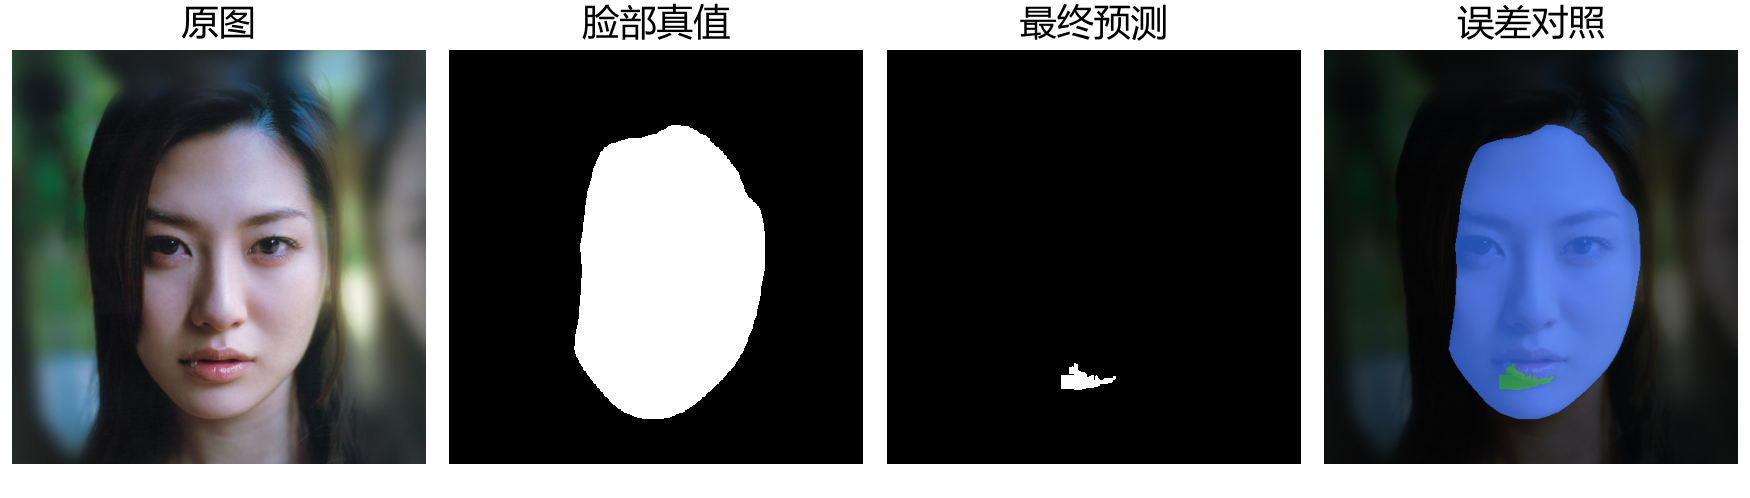
\includegraphics[width=\textwidth]{test_00609.png}
\caption{00609 的颜色候选不足导致大面积漏检}
\label{fig:test609}
\end{figure}

这张图最终 Precision 为 100\%，但 Recall 只有 1.59\%，F1 为 0.031。留下的小块全部在脸内，并不代表找回了完整脸部。图像整体偏冷，可以据此进一步检查颜色分布与训练范围的偏移，当前直接看到的失败过程是候选稀少、区域碎裂和连续丢失正确像素。

00718 则出现了另一种情况，如图~\ref{fig:test718} 所示。棕色头发形成了大块候选，最大区域选择后只有 2,705 个正确像素，却有 56,011 个误检像素。填孔又增加 10,871 个误检，只补回 110 个正确像素，最终 F1 降到 0.045。

\begin{figure}[H]
\centering
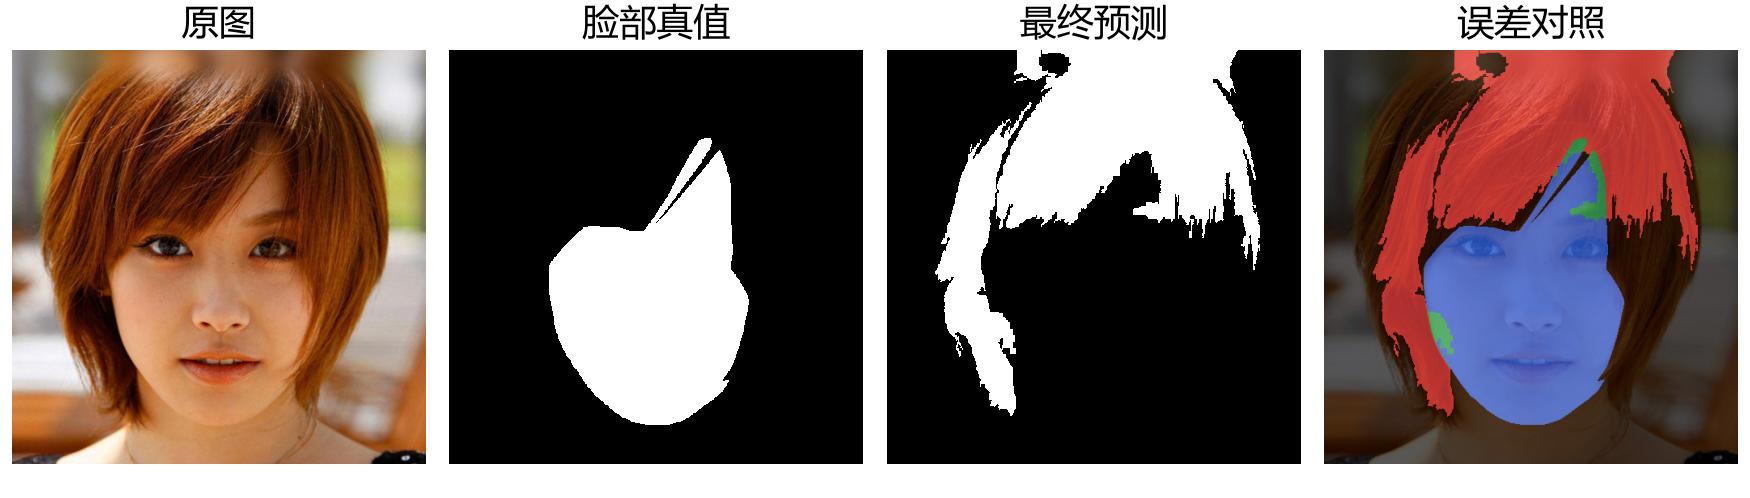
\includegraphics[width=\textwidth]{test_00718.png}
\caption{00718 中头发被选为主要候选，填孔扩大了误检}
\label{fig:test718}
\end{figure}

这时即使结果变得更连贯，所覆盖的对象仍然选错了。面积只能说明区域大小，填孔只能根据连通关系补全内部，识别候选是否属于脸部还需要更合适的判别依据。

\FloatBarrier
\subsection{误检来源与五官恢复}

将最终误检按原始标签归类，表~\ref{tab:fpclasses} 列出各类误检的计数和占比，后者以全部 FP 为分母。

\begin{table}[H]
\centering
\small
\caption{各负类的误检计数与占比}\label{tab:fpclasses}
\begin{tabular}{lrrr}
\toprule
原始类别 & 基线 FP & 最终 FP & 占最终全部 FP \\
\midrule
头发 & 772,905 & 497,516 & 60.58\% \\
脖颈 & 248,769 & 192,139 & 23.40\% \\
背景 & 369,581 & 93,639 & 11.40\% \\
衣服 & 58,056 & 20,420 & 2.49\% \\
右耳 & 9,854 & 9,574 & 1.17\% \\
左耳 & 7,811 & 4,610 & 0.56\% \\
耳饰 & 2,331 & 2,123 & 0.26\% \\
项链 & 1,189 & 1,250 & 0.15\% \\
\bottomrule
\end{tabular}
\end{table}

头发和脖颈合计占最终误检的 83.97\%。头发容易形成类肤色候选，脖颈则与脸部具有相近颜色，并可能连在同一前景块上。所以剩余问题不仅来自分离的背景，也来自与脸部相近或相连的区域。对后者继续做最大区域筛选，作用会比较有限。

另一方面，填孔确实帮助恢复了五官。将评价正类分为参与颜色建模的皮肤与鼻子，以及眼、眉、口腔与嘴唇两组，得到表~\ref{tab:facialparts} 中的组内召回率。

\begin{table}[H]
\centering
\small
\caption{不同脸部区域的召回率，单位为百分比}\label{tab:facialparts}
\begin{tabular}{lrr}
\toprule
正类分组 & 最大区域后 & 填孔后 \\
\midrule
皮肤与鼻子 & 66.43 & 76.27 \\
眼、眉、口腔与嘴唇 & 32.61 & 68.32 \\
\bottomrule
\end{tabular}
\end{table}

五官组的召回率由 32.61\% 提高到 68.32\%，共补回 69,662 个正确像素。填孔也恢复了 192,372 个皮肤与鼻子像素。完整脸部的评价目标因此需要颜色和结构共同配合，颜色负责提供主体候选，区域处理再恢复被主体包围的缺失。

\subsection{逐图稳定性与场景差异}

总体分数提高后，还需要看这种改善是否覆盖大多数图片。32 张图中有 27 张 F1 提高，5 张下降，逐图中位数由 0.664 提高到 0.778，同时最差值从 0.273 降到 0.031。最终方案对多数图像有效，少数失败却更严重。
\begin{figure}[H]
\centering
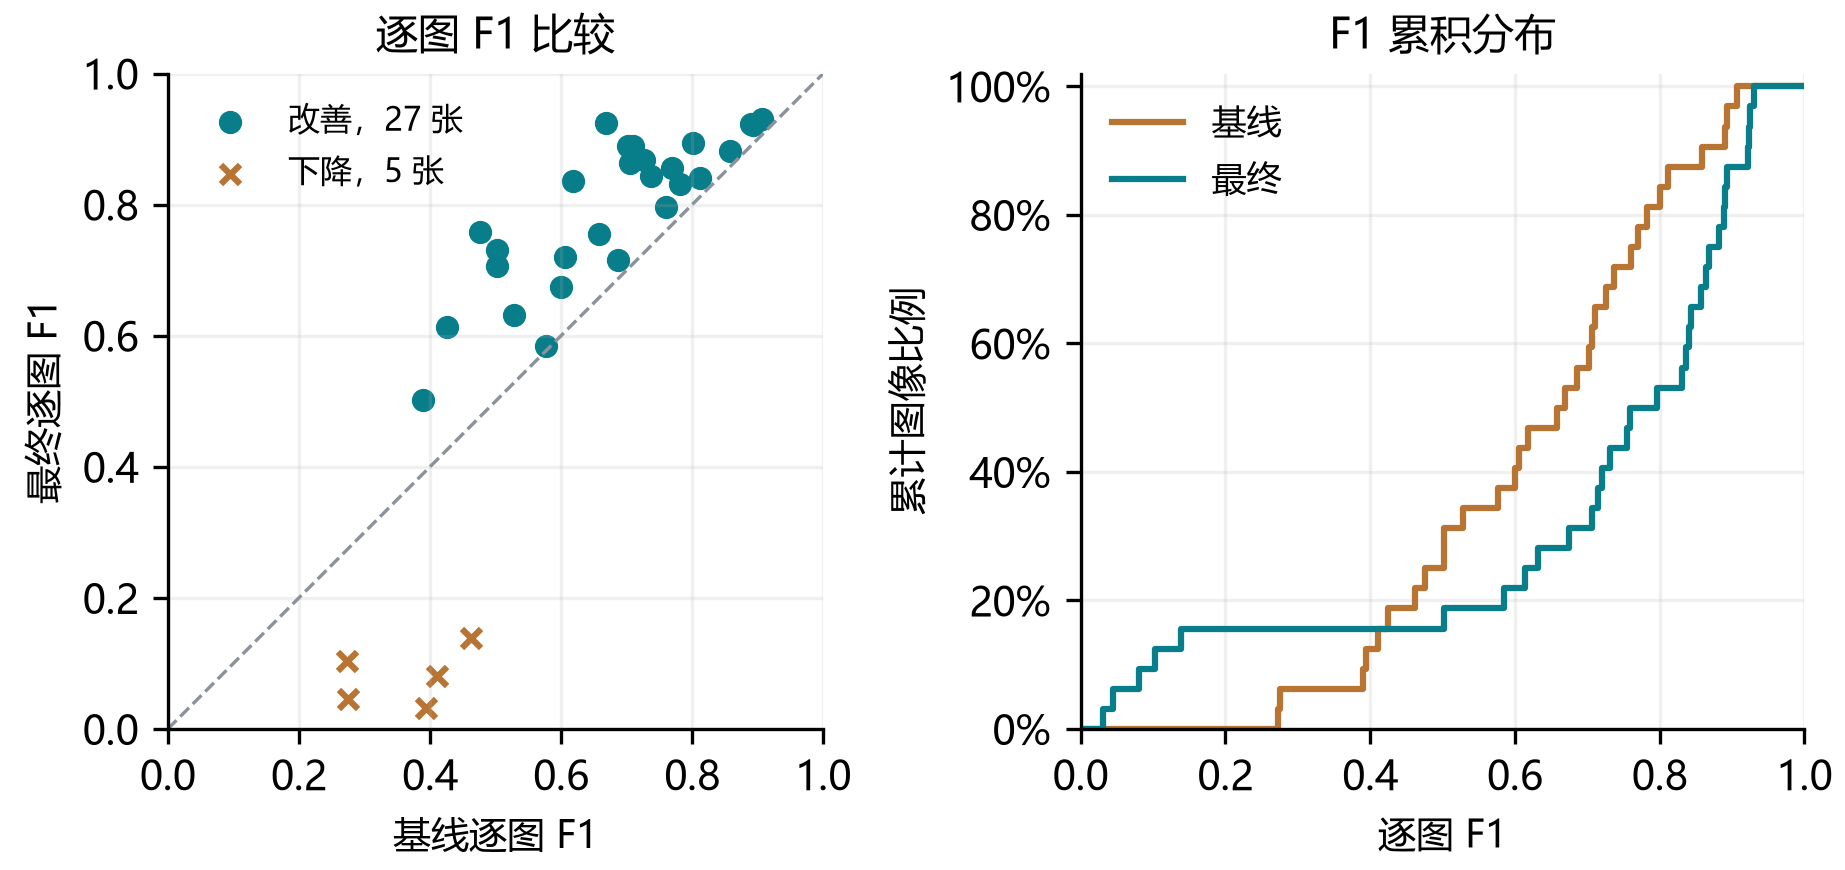
\includegraphics[width=\textwidth]{sample_stability.png}
\caption{逐图 F1 比较与累积分布}
\label{fig:samplestability}
\end{figure}

图~\ref{fig:samplestability} 左侧每个点对应一张测试图，虚线上方表示最终方案的 F1 更高。右侧纵轴表示 F1 不超过横轴数值的图像比例，可以同时看到大多数图像的变化和低分样例。

\begin{table}[H]
\centering
\small
\caption{逐图表现与边界质量}\label{tab:stability}
\begin{tabular}{lrr}
\toprule
统计项目 & 基线 & 最终 \\
\midrule
逐图 F1 平均 & 0.628 & 0.681 \\
逐图 F1 中位数 & 0.664 & 0.778 \\
逐图 F1 最小值 & 0.273 & 0.031 \\
逐图 Boundary IoU 平均 & 0.153 & 0.233 \\
\bottomrule
\end{tabular}
\end{table}

另外采用 Boundary IoU 观察轮廓贴合程度\cite{boundaryiou}。本次使用预测和真值各自的内侧边界带，带宽取图像对角线的 2\%，在当前尺寸下为 14 像素，再对逐图结果取平均。其均值由 0.153 提高到 0.233，说明区域重合改善的同时，边界也有所改善。逐图分布见图~\ref{fig:boundarydistribution}。
\begin{figure}[H]
\centering
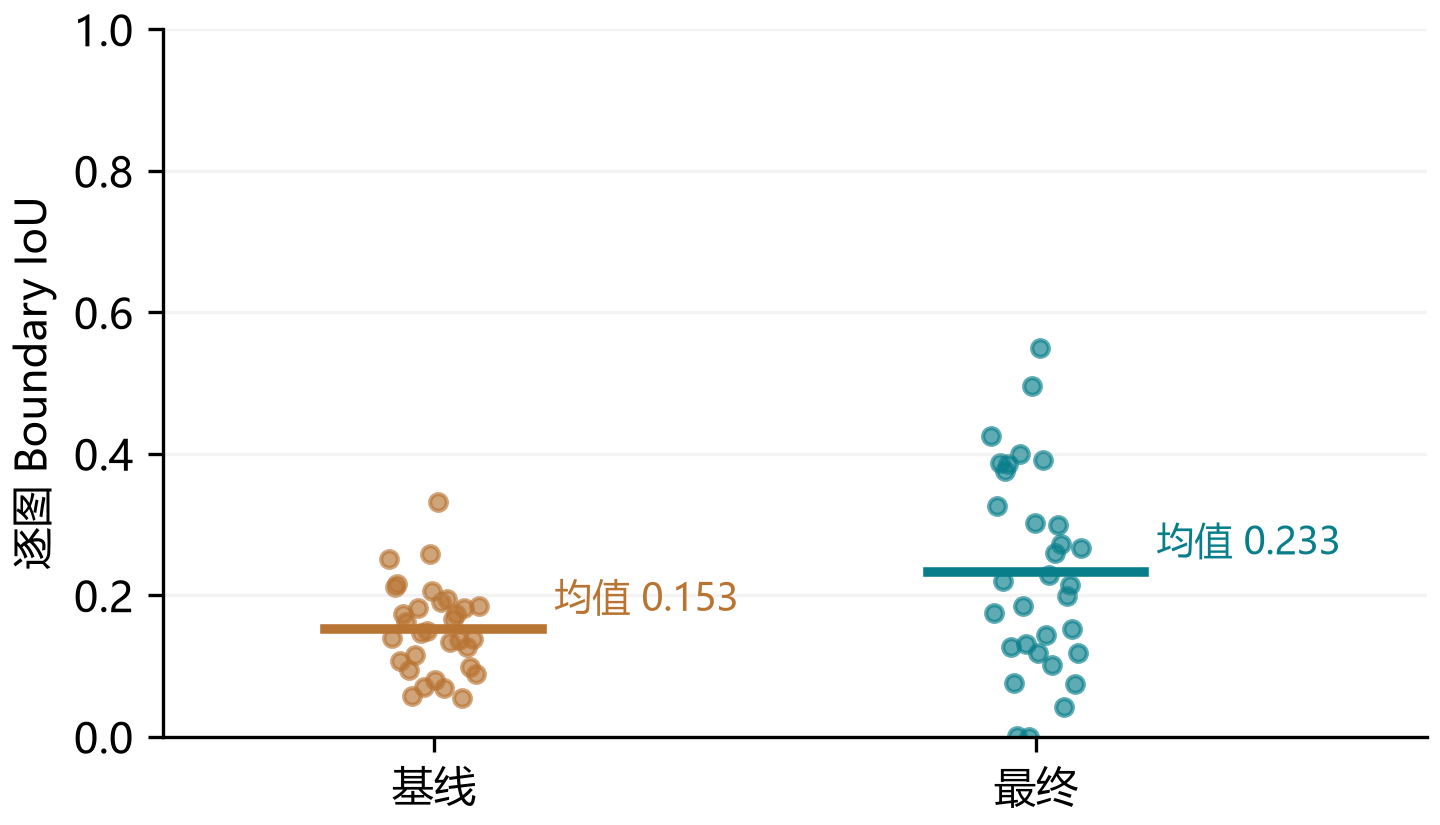
\includegraphics[width=0.78\textwidth]{boundary_distribution.png}
\caption{32 张测试图的边界质量分布，横线表示逐图均值}
\label{fig:boundarydistribution}
\end{figure}

5 张退步图在 $k=1.25$ 的原始颜色候选阶段，Recall 均低于 25\%，随后最大区域选择又丢失了部分正确碎片。因此，对严重失败图的排查应从颜色候选开始，再看区域选择保留了什么。

为了观察这批图像组成变化时改善幅度的波动，按图像配对重采样 10,000 次，使用种子 42，得到图~\ref{fig:uncertainty} 中的 95\% 区间。每次抽取相同的图像编号比较两套方案，总体 F1 先累加像素计数再计算，逐图平均 F1 则对图像等权平均。

总体 F1 差值的区间为 +3.57 至 +12.00 个百分点，逐图平均 F1 差值的区间为 -0.68 至 +10.60 个百分点。两种口径分别观察总体计数和图像平均，后者更能体现少数样例大幅退步带来的波动。这些区间描述当前 32 张图的重采样变化。

\begin{figure}[H]
\centering
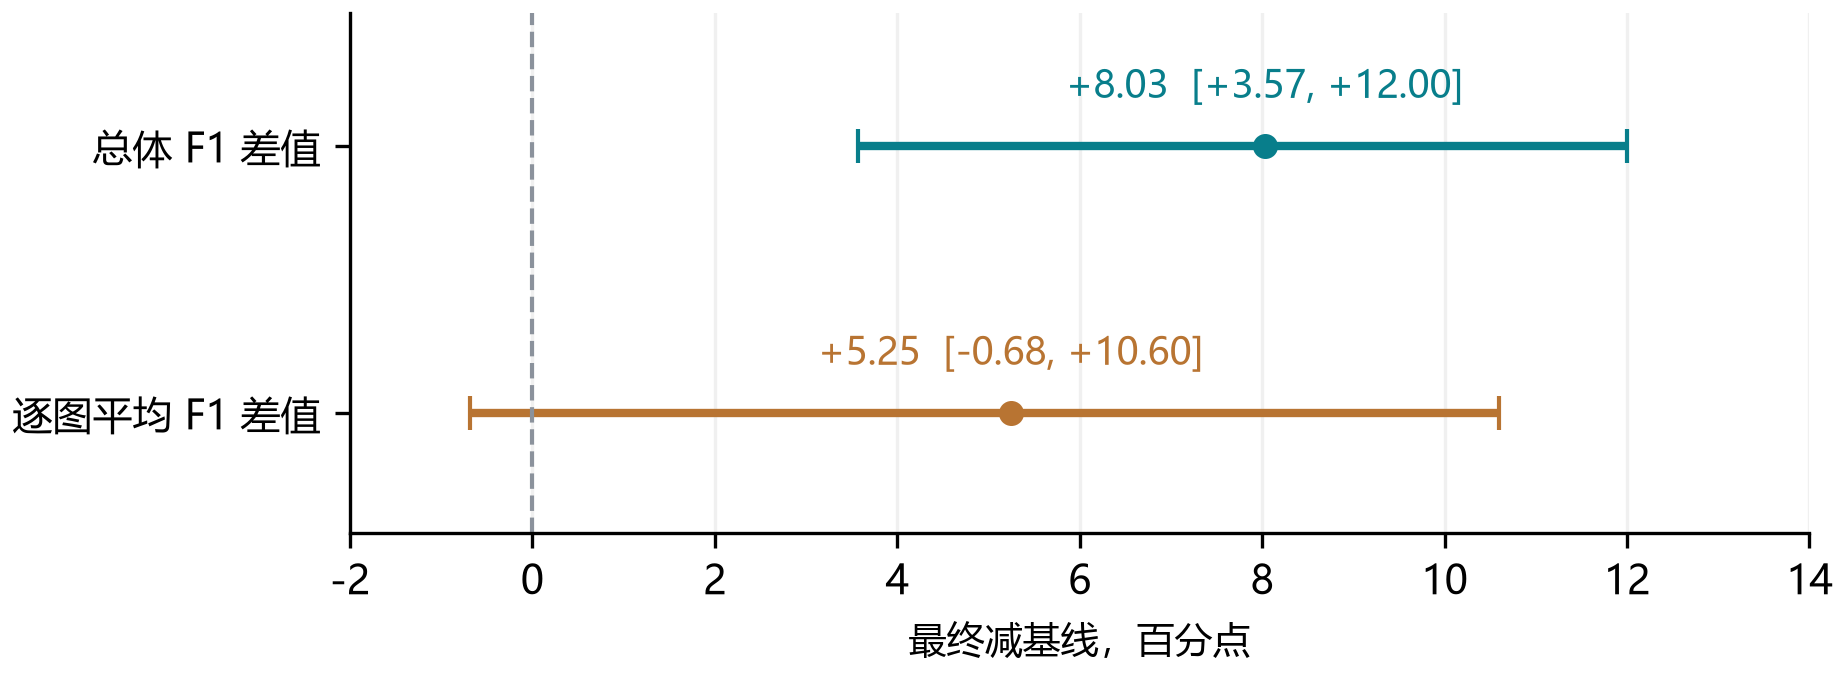
\includegraphics[width=\textwidth]{uncertainty.png}
\caption{按图像配对重采样得到的 F1 改善区间，点为观察差值，横线为 95\% 区间}
\label{fig:uncertainty}
\end{figure}

按真值脸部平均 Y 值排序，将测试图分为 11、11、10 张的较低、中间、较高亮度三组，结果见表~\ref{tab:brightness}。

\begin{table}[H]
\centering
\small
\caption{探索性亮度分组的总体 F1，单位为百分比}\label{tab:brightness}
\begin{tabular}{lrrrr}
\toprule
分组 & 图像数 & 平均 Y 范围 & 基线 F1 & 最终 F1 \\
\midrule
较低亮度 & 11 & 103.9--150.9 & 56.56 & 52.82 \\
中间亮度 & 11 & 152.4--162.7 & 61.90 & 74.88 \\
较高亮度 & 10 & 162.7--205.0 & 69.43 & 83.00 \\
\bottomrule
\end{tabular}
\end{table}

较低亮度组的 F1 由 56.56\% 降到 52.82\%，其他两组则有较大提高。这给出了进一步检查图像条件的方向。当前算法直接使用 Cr、Cb，图像的亮度、偏色和场景内容会一起影响观察结果，后续可以通过控制单一变化的实验区分它们的作用。

\subsection{改进方向与适用范围}

首先应集中检查头发和脖颈混淆。可以在训练集中补充这两类负样本的颜色分布，再比较颜色判别与位置、形状约束的组合。对于与脸部连成一块的区域，还需要考虑轮廓边界，比较时同时记录总体 F1 和这两类 FP 的变化。

其次，候选稀少或碎裂时，直接保留最大块容易继续丢失脸部。可以比较多个候选的评分或有限多区域保留，再检查是否重新引入大块背景。填孔也应结合所选区域检查，00718 的结果表明，错误候选上的填孔会扩大误检，而限制过严又可能损失五官恢复效果。

颜色模型本身还有可以利用的信息。训练统计中 Cr 与 Cb 的相关系数约为 $-0.7644$，现有矩形范围分别约束两通道，考虑联合分布是一个明确的比较方向。若进一步采用白平衡或颜色归一化，则需要统一训练与检测的处理流程，并重新计算对应统计。

这些改动可以先在验证集上逐项比较，保留每次变化的误检、漏检和典型图。当前 32 张测试图已经提供了开发线索，后续方案需要另外安排独立测试。现有数据来自外观筛选，场景和人物覆盖有限，本节结论对应当前划分，主要说明这套颜色与区域处理的收益和失败方式。
